\subsection{Scalability with Increasing Domain Size}
\label{sec:res:size}

%Domain Analyzer Time
\newtext{The exploration time to identify a domain-specific platform using our approach consists of two parts: domain analysis and design exploration. The initial domain analysis is fast: analyzing the synthetic domain with 100 apps (with up to 12 nodes each) on Intel i5-3450 with 3.10GHz takes 22.1s. Since the initial domain analysis only executes only once, this section mainly focuses on the scalability of domain exploration.} 

%Graph to show the scalability of our graph
Exploration time is correlated to the size of the domain, more specifically: the number of function types. \figref{fig:scale} analyzes the exploration time as well as the achievement over number of function types to measure scalability. 

\begin{figure}[h]
	%\vspace{-5pt}
	\centering
		%\subfloat[FT=50, diff HW budget]{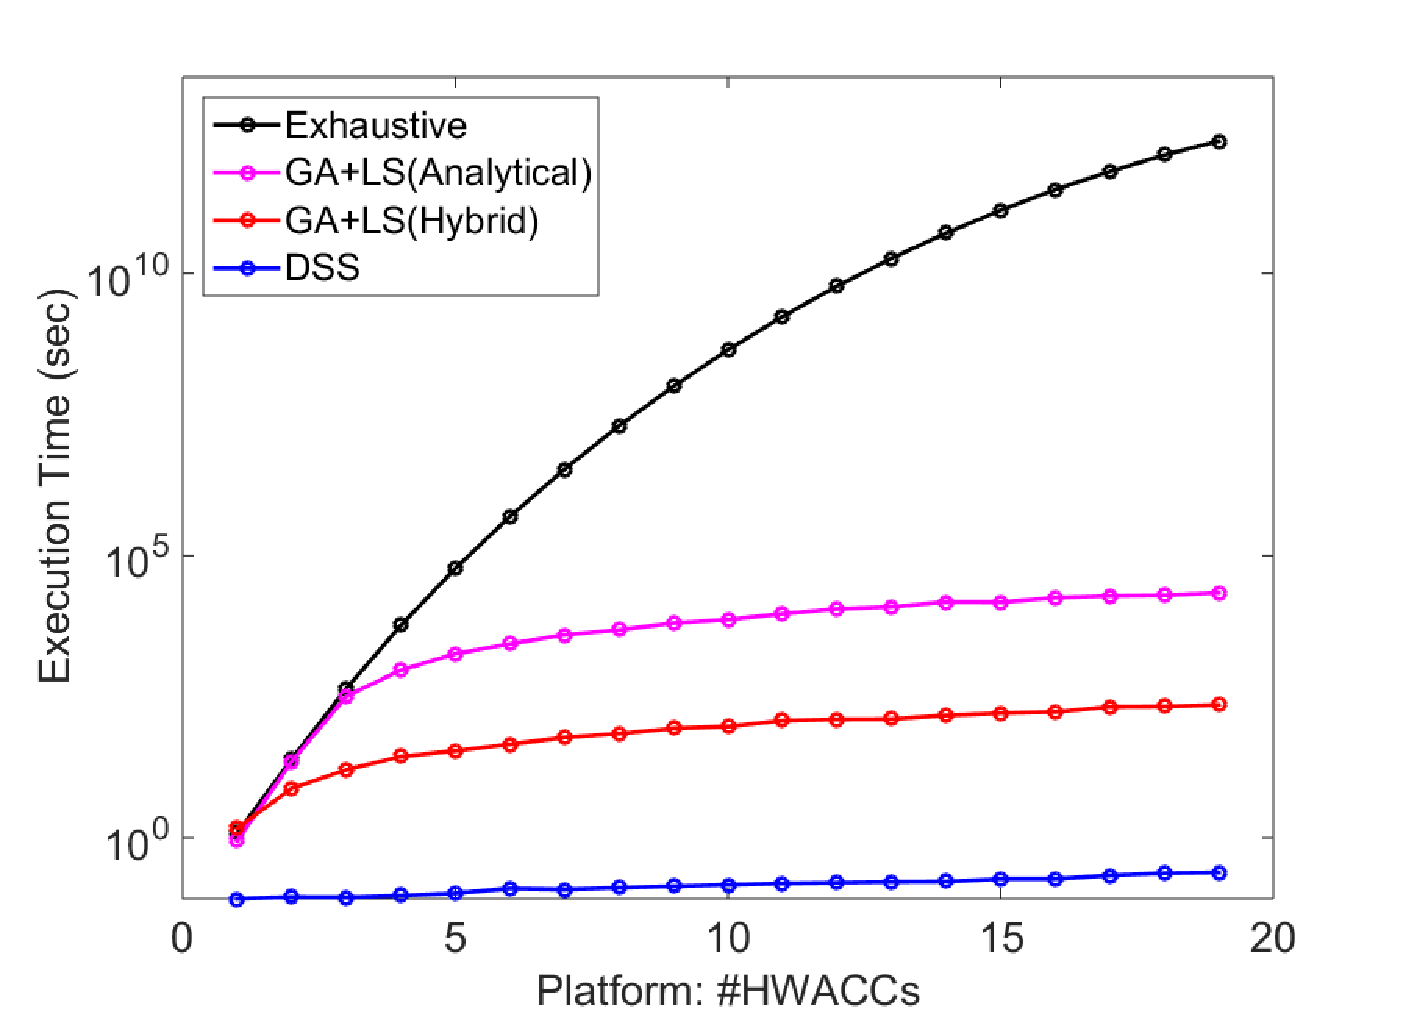
\includegraphics[width=.5\linewidth]{fig/prTimeHW.pdf}\label{fig:timeHW}}
		\subfloat[Exploration Time]{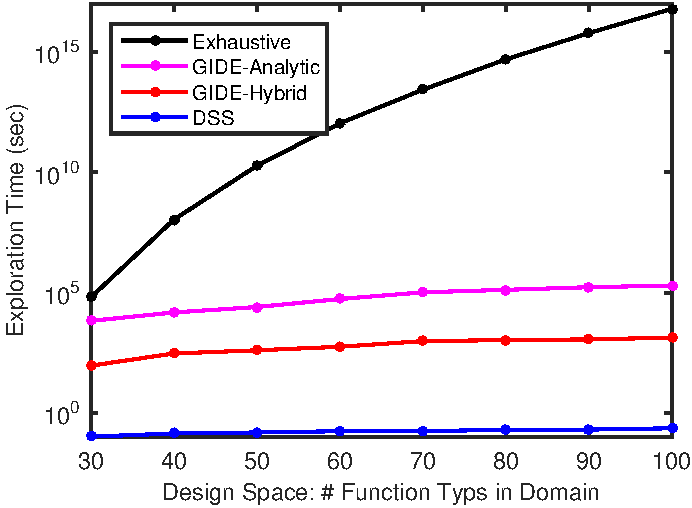
\includegraphics[width=.5\linewidth]{fig/prTimeSpace.pdf}\label{fig:timeSpace}}
		\hfill
		\subfloat[Relative Throughput]{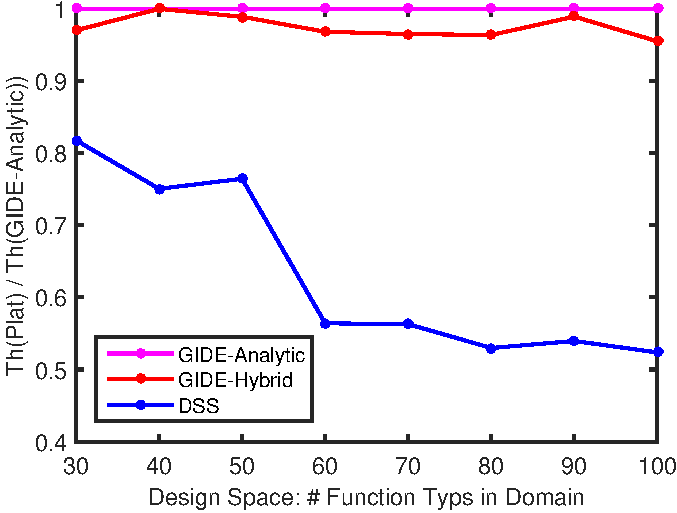
\includegraphics[width=.5\linewidth]{fig/prPASpace.pdf}\label{fig:paSpace}}
	%\vspace{-4pt}
	\caption{Scalability with Domain Size}
	\label{fig:scale}
	%\vspace{-8pt}
\end{figure}

\figref{fig:timeSpace} shows that with increasing design space, DSS and \ga scale well only slowdown linearly. The orders of magnitude comparisons hold with these approaches across size. Conversely, the Exhaustive search exponentially increases exploration time (estimation only). The benefits are most predominant with the largest domain (FT=100). Here, \gah is $4.6*10^{13}$ times faster than exhaustive.

Fig.~\ref{fig:paSpace} illustrates the stability of results over increasing domain size. However, obtaining the domain optimal platform is infeasible due to exorbitant long exploration time ($3*10^8$ years, FT=100). As an approximation, \figref{fig:paSpace} shows relative throughput compared to \gaana. Even over large domains \gah scales very well and its results remain close to \gaana with 97.51\% on average. Conversely, the limitations of DSS become more pronounced as domain size increases (63.16\%).

%Performance over increasing domain size. The first graph should be changed to performance versus time.
%\begin{figure}[H]
%	\centering
%		\subfloat[Relative Throughput]{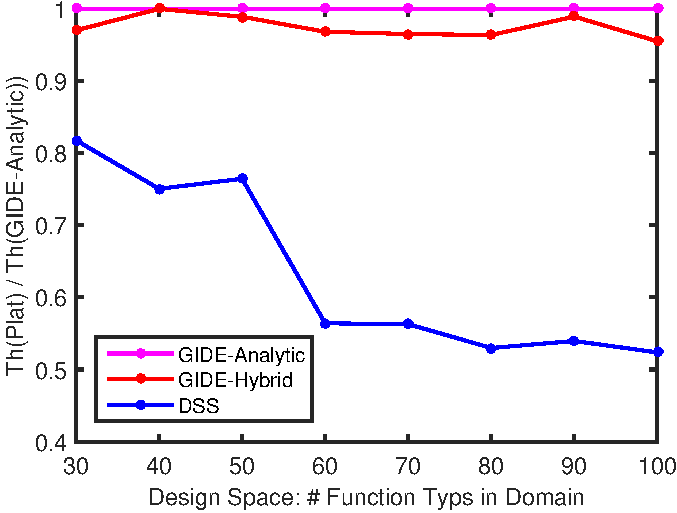
\includegraphics[width=.5\linewidth]{fig/prPASpace.pdf}\label{fig:paSpace}}
%		\hfill
%		\subfloat[Performance vs Time]{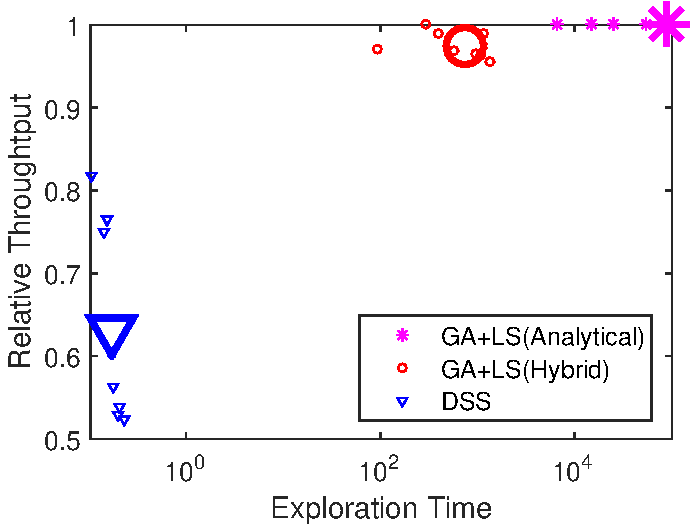
\includegraphics[width=.5\linewidth]{fig/prPATimeSpace.pdf}\label{fig:paTimeSpace}}
%	\caption{Synthetic Domain: HW=19, with diff design space}
%\end{figure}

%Fig.~\ref{fig:paTimeSpace} trade-off. GA Hybrid could achieve high performance, with less exploring time compared with GA-analytical. Although the DSS is much faster than other two algorithm, it could get the good domain platform.